\documentclass[12pt]{article}

\usepackage{fullpage}
\usepackage{mdframed}
\usepackage{multicol}
\usepackage{colonequals}
\usepackage{algpseudocode}
\usepackage{algorithm}
\usepackage[most, breakable]{tcolorbox}
\usepackage[all]{xy}
\usepackage{proof}
\usepackage{mathtools}
\usepackage{bbm}
\usepackage{amssymb}
\usepackage{amsthm}
\usepackage{amsmath}
\usepackage{amsxtra}
\usepackage{tikz-cd}
\usepackage{enumitem}
\usepackage{euler}
\usepackage{mathpazo}
\usepackage{wrapfig}

\newtheorem{theorem}{Theorem}[section]
\newtheorem{theorem*}{Theorem}
\newtheorem{definition}[theorem]{Definition}
\newtheorem{corollary}{Corollary}[theorem]
\newtheorem{lemma}[theorem]{Lemma}
\newtheorem{lemmact}[theorem]{Lemmact}
\newtheorem{proposition}[theorem]{Proposition}
\newtheorem{remark}[theorem]{Remark}
\newtheorem{example}{Example}[section]


% \newtheorem*{exercisehelper}{Exercise.}
% \newenvironment{exercise}[1]{%
%   \IfBlankTF{#1}
%     {\renewcommand{\exercisehelper}{\textbf{Exercise} \unskip}}
%     {\renewcommand\exercisehelper{\textbf{Exercise #1}}}%
%   \exercisehelper
% }{\endexercisehelper}

\theoremstyle{remark}
\newtheorem{exercise}{Exercise}[section]
\newtheorem*{solution}{Solution}
\newtheorem*{notation}{Notation}
\newcommand{\mathcat}[1]{\textup{\textbf{\textsf{#1}}}} % for defined terms

\newenvironment{problem}[1]
{ \begin{tcolorbox}[breakable]\noindent\textbf{Problem #1}.}
{\vskip 6pt \end{tcolorbox}}

\newenvironment{enumalph}
{\begin{enumerate}\renewcommand{\labelenumi}{\textnormal{(\alph{enumi})}}}
{\end{enumerate}}

\newenvironment{enumroman}
{\begin{enumerate}\renewcommand{\labelenumi}{\textnormal{(\roman{enumi})}}}
{\end{enumerate}}

\newcommand{\defi}[1]{\textsf{#1}} % for defined terms



\setlength{\hfuzz}{4pt}

\let\H\relax
\let\P\relax
\newcommand{\bb}{\mathbb}
\newcommand{\A}{\mathbb A}
\newcommand{\H}{\mathbb H}
\newcommand{\E}{\mathbb E}
\newcommand{\P}{\mathbb P}
\newcommand{\C}{\mathbb C}
\newcommand{\I}{\mathbb I}
\newcommand{\K}{\mathbb K}
\newcommand{\N}{\mathbb N}
\newcommand{\Q}{\mathbb Q}
\newcommand{\R}{\mathbb R}
\newcommand{\Z}{\mathbb Z}
\newcommand{\F}{\mathbb F}
\newcommand{\V}{\mathbb V}
\newcommand{\br}{\mathbf{r}}
\newcommand{\RP}{\mathbb{RP}}
\newcommand{\CP}{\mathbb{CP}}
\newcommand{\nbit}[1]{\{0, 1\}^{#1}}
\newcommand{\bits}{\{0, 1\}^{n}}
\newcommand{\bbni}{\bigbreak \noindent}
\newcommand{\norm}[1]{\left\vert\left\vert#1\right\vert\right\vert}
\newcommand{\dbar}{\overline{\partial}}
\let\d\relax
\newcommand{\d}{\partial}
\newcommand{\e}{\epsilon}
\newcommand{\cO}{\mathcal{O}}
\newcommand{\FF}{\mathcal{F}}
\newcommand{\cG}{\mathcal{G}}
\newcommand{\HH}{\mathcal{H}}
\newcommand{\EE}{\mathcal{E}}
\newcommand{\CC}{\mathcal{C}}
\newcommand{\DD}{\mathcal{D}}
\newcommand{\PP}{\mathcal{P}}
\newcommand{\iso}{\cong}
\newcommand{\tism}{Talked to Sair Shaikh'26}
\DeclareMathOperator{\fm}{\mathfrak{m}}
\DeclareMathOperator{\fn}{\mathfrak{n}}
\DeclareMathOperator{\fp}{\mathfrak{p}}
\DeclareMathOperator{\fq}{\mathfrak{q}}
\DeclareMathOperator{\fM}{\mathfrak{M}}
\DeclareMathOperator{\fP}{\mathfrak{P}}


\newcommand{\Frac}{\text{Frac}}
\newcommand{\Tor}{\text{Tor}}
\newcommand{\Ext}{\text{Ext}}
\newcommand{\gr}{\text{gr}}
\newcommand{\pd}{\text{pd}}
\newcommand{\Proj}{\text{Proj}}
\newcommand{\NF}{\text{NF}}
\newcommand{\Jac}{\text{Jac}}
\newcommand{\red}{\text{red}}
\newcommand{\Nil}{\text{Nil}}
\newcommand{\LC}{\text{LC}}
\newcommand{\LM}{\text{LM}}
\newcommand{\LT}{\text{LT}}
\newcommand{\GL}{\text{GL}}
\newcommand{\tp}{\text{T}}
\newcommand{\init}{\text{in}}
\DeclareMathOperator{\Bl}{Bl}


\DeclareMathOperator{\cS}{\mathscr S}
\DeclareMathOperator{\cV}{\mathscr V}
\DeclareMathOperator{\cR}{\mathscr R}
\DeclareMathOperator{\cT}{\mathscr T}
\DeclareMathOperator{\comRing}{\textbf{comRing}}
\DeclareMathOperator{\Ann}{\text{Ann}}
\DeclareMathOperator{\adj}{\text{Adj}}
\DeclareMathOperator{\Top}{\textbf{Top}}
\DeclareMathOperator{\Mod}{\textbf{Mod}}
% \renewcommand{\Top}{\textbf{Top}}
\DeclareMathOperator{\Set}{\textbf{Set}}
\DeclareMathOperator{\alg}{\textbf{alg}}
\DeclareMathOperator{\ord}{\textbf{ord}}
\DeclareMathOperator{\height}{\text{ht}}
\DeclareMathOperator{\trdeg}{\text{tr.deg}}
\DeclareMathOperator{\std}{\text{std}}
\DeclareMathOperator{\depth}{\text{depth}}
\DeclareMathOperator{\ini}{\text{in}}




\let\1\relax
\newcommand{\1}{\mathbf{1}}
\newcommand{\fr}[2]{\left(\frac{#1}{#2}\right)}
\newcommand{\todo}[1]{\textcolor{red}{\textbf{TODO:} #1}}
\newcommand{\vecz}{\mathbf{z}}
\newcommand{\vecr}{\mathbf{r}}
\DeclareMathOperator{\ot}{\leftarrow}
\DeclareMathOperator{\Cinf}{C^{\infty}}
\DeclareMathOperator{\Id}{Id}
\DeclareMathOperator{\Ell}{Ell}
\DeclareMathOperator{\CL}{\mathcal{CL}}
\DeclareMathOperator{\Alt}{Alt}
\DeclareMathOperator{\Aut}{Aut}
\DeclareMathOperator{\ann}{ann}
\DeclareMathOperator{\codim}{codim}
\DeclareMathOperator{\End}{End}
\DeclareMathOperator{\Hom}{Hom}
\DeclareMathOperator{\id}{id}
\DeclareMathOperator{\im}{im}
\DeclareMathOperator{\M}{M}
\DeclareMathOperator{\Mat}{Mat}
\DeclareMathOperator{\Ob}{Ob}
\DeclareMathOperator{\opchar}{char}
\DeclareMathOperator{\opspan}{span}
\DeclareMathOperator{\rk}{rk}
\DeclareMathOperator{\ev}{ev}
\DeclareMathOperator{\sgn}{sgn}
\DeclareMathOperator{\Sym}{Sym}
\DeclareMathOperator{\tr}{tr}
\DeclareMathOperator{\img}{img}
\DeclareMathOperator{\coker}{coker}
\DeclareMathOperator{\Spec}{Spec}
\DeclareMathOperator{\mSpec}{mSpec}
\DeclareMathOperator{\CandE}{CandE}
\DeclareMathOperator{\CandO}{CandO}
\DeclareMathOperator{\argmax}{argmax}
\DeclareMathOperator{\first}{first}
\DeclareMathOperator{\last}{last}
\DeclareMathOperator{\cost}{cost}
\DeclareMathOperator{\dist}{dist}
\DeclareMathOperator{\path}{path}
\DeclareMathOperator{\parent}{parent}
\DeclareMathOperator{\argmin}{argmin}
\DeclareMathOperator{\excess}{excess}
\let\Pr\relax
\DeclareMathOperator{\Pr}{\mathbf{Pr}}
\DeclareMathOperator{\Exp}{\mathbb{E}}
\DeclareMathOperator{\Var}{\mathbf{Var}}
\let\limsup\relax
\DeclareMathOperator{\limsup}{limsup}
%Paired Delims
\DeclarePairedDelimiter\ceil{\lceil}{\rceil}
\let\oldceil\ceil
\renewcommand{\ceil}[1]{\oldceil*{#1}}

\DeclarePairedDelimiter{\floor}{\lfloor}{\rfloor}
\let\oldfloor\floor
\renewcommand{\floor}[1]{\oldfloor*{#1}}


\newcommand{\circled}[2][]{
  \tikz[baseline=(char.base)]{
    \node[shape=circle, draw, inner sep=1.5pt, #1] (char) {$#2$};
  }
}
\newcommand{\dcircled}[2][]{
  \tikz[baseline=(X.base)]{
    \node[circle, draw, double, double distance=2pt, inner sep=1.5pt, #1] (X) {$#2$};
  }
}

\newcommand{\dagstar}{*}

\newcommand{\tbigwedge}{{\textstyle{\bigwedge}}}
\setlength{\parindent}{0pt}
\setlength{\parskip}{5pt}


\usepackage{listings}
\usepackage{courier}
\usepackage{microtype}


\lstset{
  basicstyle=\footnotesize\ttfamily,
  breaklines=true,
  breakatwhitespace=true
  columns=fullflexible,
  keepspaces=true,
  frame=single,
  escapeinside={(*@}{@*)}
}
\usepackage{pdfpages}
\usepackage{needspace}

\begin{document}

\title{COSC 42: Distributed Computing}

\author{}
\date{}
\maketitle
\vspace{-.8in}


% \begin{problem}{0. Learn TLA+ (Required)}

% Follow {https://lamport.azurewebsites.net/video/videos.html} to learn TLA+ and how to use the TLC Model Checker. The video course will walk you through the use of the TLA+ toolbox. Make sure to give yourself a lot of time to go through these videos. The videos have intermittent exercises to help you learn and confirm your understanding, so you may often need to pause the video, think, go through an exercise, re-watch an earlier video, or seek help if you get stuck somewhere.
% \end{problem}

\begin{problem}{1. Model Checking Peterson's Algorithm}

Specify Peterson's Algorithm in TLA+. Formulate Mutual Exclusion of Peterson's Algorithm as an invariant. Use the TLC Model Checker to prove (by exhaustive search) that Peterson's Algorithm satisfies Mutual Exclusion.
\end{problem}

\begin{solution}
    \bbni
    
    TLC exhaustively found all 66 (32 distinct) reachable states and found no violation of Mutex. Thus, the model satisfies mutual exclusion.

  \begin{tcolorbox}[title={TLA+ model},boxsep=0pt,
    left=3pt,right=3pt,top=3pt,bottom=3pt]
\centering
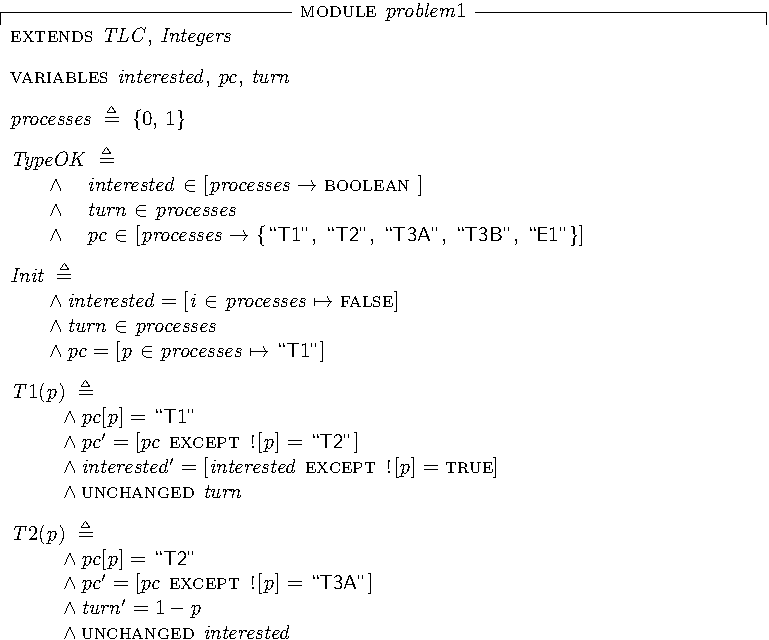
\includegraphics[page=1,width=0.9\linewidth]
    {TLA/problem1-cropped.pdf}\par
\end{tcolorbox}

\begin{tcolorbox}[title={TLA+ model continued},boxsep=0pt,
    left=3pt,right=3pt,top=3pt,bottom=3pt]
\centering
\includegraphics[page=2,width=0.9\linewidth]
    {TLA/problem1-cropped.pdf}\par
\end{tcolorbox}

\tcbinputlisting{
    title={TLC configuration},
    listing file={TLA/problem1.cfg},
    listing only,
    breakable,
    listing options={
        language={},
        basicstyle=\small\ttfamily,
        columns=fullflexible,
        keepspaces=true,
        breaklines=true,
        frame=none,
        escapeinside={},
        mathescape=false
    }
}
\end{solution}

\newpage

\begin{problem}{2. Puli Meka Gaddi}

The following is a Telugu folk puzzle called \emph{Puli Meka Gaddi} (translating to \emph{Tiger, Goat, and Hay}).

A boatman has a tiger, a goat, and a bale of hay and is on the left bank of a river. His objective is to cross from the left bank of the river to the right bank of the river and to end up on the right bank of the river with all of his three life-forms (tiger, goat, and hay). Unfortunately, his boat only has space for him and one of the three life-forms, therefore he can take at most one of the life-forms with him in the boat at a time. Thus, he must necessarily make several left-to-right and right-to-left trips across the river to achieve his goal. In addition, the boatman also faces the following conundrum, if he leaves the tiger and goat alone together (without him), the tiger will eat the goat. Similarly, if he leaves the goat and hay alone together, the goat will eat the hay. The Puli Meka Gaddi Puzzle is to find a way for the boatman to successfully end up on the right bank of the river along with the tiger, the goat, and the hay without anything getting eaten.

In this problem, your objective is not just to solve the Puli Meka Gaddi puzzle, but to actually make the TLC model checker solve the puzzle for you. In particular, recall that the TLC model checker can check for invariants in TLA+ model specifications. Can you figure out how to use the TLC model checker to solve Puli Meka Gaddi for you?

In particular, you should specify the Puli Meka Gaddi system as a TLA+ model and formulate an appropriate non-invariant, such that model checking your non-invariant in TLC will lead the model checker to throw an ``error'' trace that is a solution to the Puli Meka Gaddi Puzzle. Submit your pretty-printed TLA+ model and the solution returned by TLC, along with a translation of the solution returned by TLC into plain English.
\end{problem}

\begin{solution}
\begin{tcolorbox}[
    title={TLA+ model},
    breakable,
    boxsep=2pt,
    left=2pt,
    right=2pt
]
    \centering
    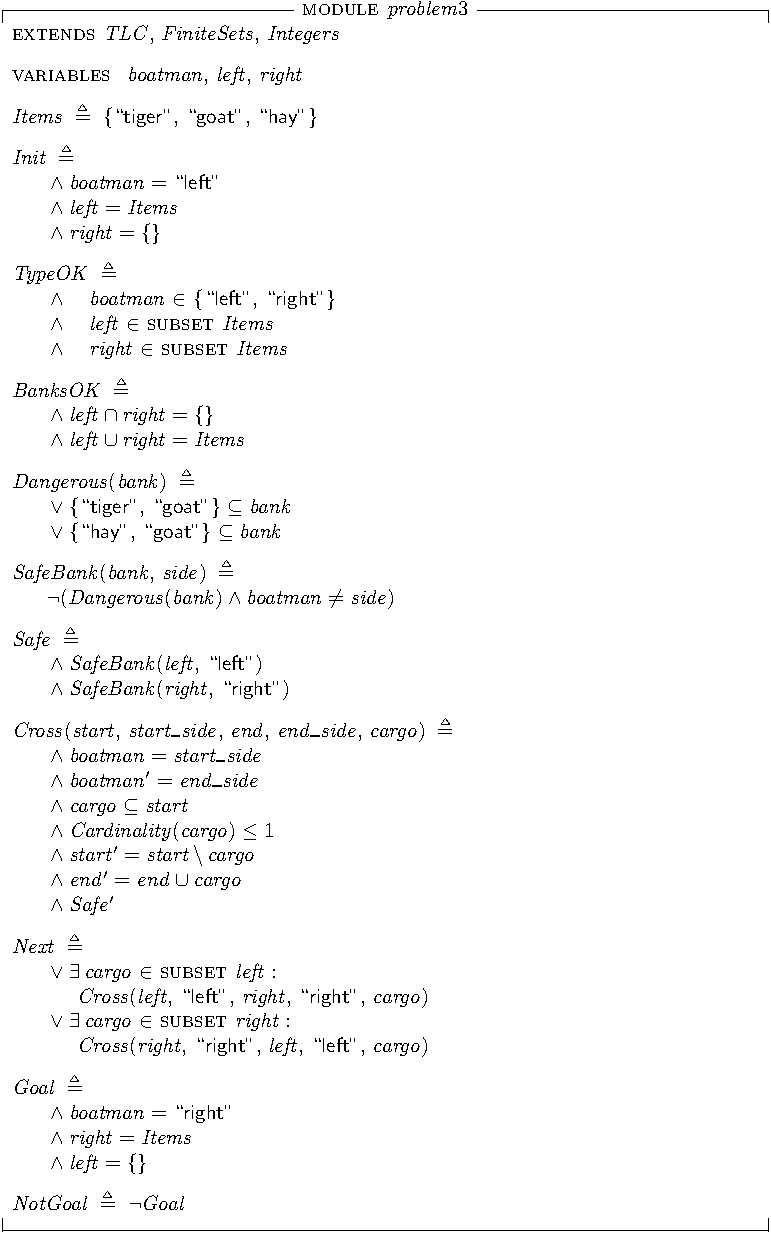
\includegraphics[
        page=1,
        width=\linewidth,
        height=0.9\textheight,
        keepaspectratio
    ]{TLA/problem3-cropped.pdf}
\end{tcolorbox}
\tcbinputlisting{
    title={TLC configuration},
    listing file={TLA/problem3.cfg},
    listing only,
    breakable,
    listing options={
        language={},
        basicstyle=\small\ttfamily,
        columns=fullflexible,
        keepspaces=true,
        breaklines=true,
        frame=none,
        escapeinside={},
        mathescape=false
    }
}
\bbni

\textbf{Solution returned by TLC:}
\tcbinputlisting{
    title={Solution returned by TLC},
    listing file={TLA/problem3-trace.txt},
    listing only,
    breakable,
    listing options={
        language={},
        basicstyle=\small\ttfamily,
        columns=fullflexible,
        keepspaces=true,
        breaklines=true,
        frame=none,
        escapeinside={},
        mathescape=false
    }
}
\bbni

\textbf{English explanation:}

We can solve the puzzle by following the following steps: 
\begin{itemize}
    \item Step 0: They all start on the left bank of the river. 
    \item Step 1: The boatman crosses to the right bank with the goat, drops it there and goes back to the left bank. 
    \item Step 2: The boatman crosses to the right bank with the tiger, drops it there, and brings the goat back to the left bank.  
    \item Step 3: The boatman crosses to the right bank with the hay, drops it there, and goes back to the left bank.  
    \item Step 4: The boatman crosses to the right bank with the goat.
\end{itemize} 
Thus successfully ending up on the right bank of the river along with the tiger, the goat, and the hay without anything getting eaten.
\end{solution}


\end{document}